\RequirePackage{fix-cm}
\documentclass[oneside, a4paper]{book}
\usepackage[a4paper,width=150mm,top=25mm,bottom=25mm,bindingoffset=6mm]{geometry}

% Required for inserting images
\usepackage{eso-pic,graphicx}
% misc
\usepackage{caption}
\DeclareCaptionType{equ}[][]
%\captionsetup[equ]{labelformat=empty}
\usepackage{subcaption}
\usepackage{multicol}
\usepackage{float}
\usepackage{adjustbox} % oversized table

% appendix
\usepackage[toc]{appendix}

% Default font to sans serif
\renewcommand{\familydefault}{\sfdefault}
\RequirePackage[T1]{fontenc} 
\RequirePackage[tt=false, type1=true]{libertine} 
\RequirePackage[varqu]{zi4} 
% \RequirePackage[libertine]{newtxmath}

% chapters and headers
\usepackage[Conny]{fncychap}

\usepackage{fancyhdr}
\pagestyle{fancy}
\renewcommand{\headrulewidth}{0.1pt}
\renewcommand{\chaptermark}[1]{\markboth{\MakeUppercase{\textsf{{#1}}}}{}}
\renewcommand{\sectionmark}[1]{\markright{\MakeUppercase{\textsf{\thesection\ #1}}}{} }

% section styling
\usepackage{titlesec}

% algorithms
\usepackage{algorithm}
\usepackage{algpseudocode}

% theorems and definitions
\usepackage{amsthm}
\newtheorem{definition}{Definition}

% better tables
\usepackage{tabu}

% FAT FONTS
\usepackage{bm} % bold fonts in math mode
\newcommand\fat[1]{{\boldmath{\textbf{#1}}}}
\newcommand\emphasis[1]{{\scshape\bfseries#1}}

% mathematical fonts and graphics
\usepackage{mathtools}
\usepackage{xfrac} % sfrac for diagonal slashes in fractions
\usepackage{amsfonts} % math fonts
\usepackage{amssymb} % more math symbols (supsetneq etc.)
\usepackage{dbnsymb}
\usepackage{dsfont} % math fonts
\usepackage{bbm} % mathbb fonts
\usepackage{mathrsfs} % fancy swirly font
\usepackage{gensymb} % degree sign

% draw graphs
\usepackage[inline]{asymptote}
\usepackage{qtree}
\usepackage{tikz}
\usetikzlibrary{calc}

% nicer fractions
\usepackage{xfrac}
% cancel terms
\usepackage{cancel}

% units
\usepackage{siunitx}

% plots
\usepackage{pgfplots}
\usepackage{pgfplotstable}
\usepgfplotslibrary{external}
\usepgfplotslibrary{patchplots}
\usepgfplotslibrary{groupplots}
\pgfplotsset{compat=1.18} 
\tikzexternalize[prefix=tikz,optimize=false]

% define the Spectral_r color scheme
\usepackage[table, dvipsnames]{xcolor}
\definecolor{Spectral0}{RGB}{158, 1, 66}
\definecolor{Spectral1}{RGB}{213, 62, 79}
\definecolor{Spectral2}{RGB}{244, 109, 67}
\definecolor{Spectral3}{RGB}{253, 174, 97}
\definecolor{Spectral4}{RGB}{254,224,139}
\definecolor{Spectral5}{RGB}{255,255,191}
\definecolor{Spectral6}{RGB}{230,245,152}
\definecolor{Spectral7}{RGB}{171,221,164}
\definecolor{Spectral8}{RGB}{102,204,204}
\definecolor{Spectral9}{RGB}{50,136,189}
\definecolor{Spectral10}{RGB}{94,79,162}
\pgfplotsset{
  colormap={Spectral_r}{
    rgb255(0cm)=(94,79,162)         % 0.0
    rgb255(1cm)=(50,136,189)        % 0.1
    rgb255(2cm)=(102,204,204)       % 0.2
    rgb255(3cm)=(171,221,164)       % 0.3
    rgb255(4cm)=(230,245,152)       % 0.4
    rgb255(5cm)=(255,255,191)       % 0.5
    rgb255(6cm)=(254,224,139)       % 0.6
    rgb255(7cm)=(253,174,97)        % 0.7
    rgb255(8cm)=(244,109,67)        % 0.8
    rgb255(9cm)=(213,62,79)         % 0.9
    rgb255(10cm)=(158,1,66)         % 1.0
    }
}


% get width of given text
\usepackage{calc}

% define a horizontal spacer
\newcommand\horizontalspacer[0]{\vspace{5pt}\noindent\textcolor{lightgray}{\rule{\textwidth}{1mm}}
\vspace{5pt}}

% clickable links
\usepackage{hyperref}
\hypersetup{
    colorlinks,
    citecolor=black,
    filecolor=black,
    linkcolor=black,
    urlcolor=black
}
\renewcommand{\itemautorefname}{Item}
% fancy boxes
\usepackage{fancybox}
\newcommand{\equationnamed}[2]{%
  \setlength{\fboxsep}{2pt} % padding inside box
  \setlength{\fboxrule}{0.01pt}
  \begin{center}
    \begin{minipage}{\textwidth}
      \begin{center}\textsc{#1}\end{center}
      #2
    \end{minipage}
  \end{center}
}
\newcommand{\equationnamedbox}[2]{%
  \setlength{\fboxsep}{5pt} % padding inside box
  \setlength{\fboxrule}{0.01pt}
  \begin{center}
    \fbox{
      \begin{minipage}{0.4\textwidth}
        \begin{center}\emphasis{#1}\end{center}
        #2
      \end{minipage}
    }
  \end{center}
}

% labels to enum items
\usepackage{enumitem}

\usepackage{array}

% make empty lines skip
% \usepackage{parskip}

% include pdfs 
\usepackage{pdfpages}

% code
\usepackage{minted}
\usepackage{listings}

% ~~~~~~~~~ TYPESETTING AND OTHER MACROS ~~~~~~~~~~~~~~~~~~~~~

\newenvironment{absolutelynopagebreak}
  {\par\nobreak\vfil\penalty0\vfilneg
   \vtop\bgroup}
  {\par\xdef\tpd{\the\prevdepth}\egroup
   \prevdepth=\tpd}

% ~~~~~~~~~ AFANCY CHAPTER HEADINGS ~~~~~~~~~~~~~~~~~~~~~~~~~~~
\makeatletter
\def\thickhrulefill{\leavevmode \leaders \hrule height 1ex \hfill \kern \z@}
\def\@makechapterhead#1{%
  %\vspace*{50\p@}%
  \vspace*{10\p@}%
  {\parindent \z@ \centering \reset@font
        \thickhrulefill\quad
        \scshape \@chapapp{} \thechapter
        \quad \thickhrulefill
        \par\nobreak
        \vspace*{10\p@}%
        \interlinepenalty\@M
        \hrule
        \vspace*{10\p@}%
        \Huge {\textbf{#1}} \par\nobreak
        \par
        \vspace*{10\p@}%
        \hrule
    \vskip 40\p@
    % \vskip 100\p@
  }}
\def\@makeschapterhead#1{%
  %\vspace*{50\p@}%
  \vspace*{10\p@}%
  {\parindent \z@ \centering \reset@font
        \thickhrulefill
        \par\nobreak
        \vspace*{10\p@}%
        \interlinepenalty\@M
        \hrule
        \vspace*{10\p@}%
        \Huge \bfseries #1\par\nobreak
        \par
        \vspace*{10\p@}%
        \hrule
    \vskip 40\p@
    % \vskip 100\p@
  }}

  \newcommand*{\@rowstyle}{}
  \newcommand*{\rowstyle}[1]{% sets the style of the next row
    \gdef\@rowstyle{#1}%
    \@rowstyle\ignorespaces%
  }
  \newcolumntype{=}{% resets the row style
    >{\gdef\@rowstyle{}}%
  }
  \newcolumntype{+}{% adds the current row style to the next column
    >{\@rowstyle}%
  }
  
\usepackage[pdftex,outline]{contour}

% ~~~~~~~~~ MATH MACROS ~~~~~~~~~~~~~~~~~~~~~~~~~~~~~~~~~~~~~~

% abs value macro
% \DeclarePairedDelimiter\abs{\lvert}{\rvert}
\newcommand\abs[1]{\left|#1\right|}
\newcommand\abss[1]{\left|\left|#1\right|\right|}
\newcommand\norm[1]{\left\lVert#1\right\rVert}
\newcommand\angled[1]{\left\langle#1\right\rangle}
\newcommand\round[1]{\left\lfloor#1\right\rceil}

\newcommand\dist[1]{\left|\left|#1\right|\right|}
\newcommand\arr[1]{\left\langle#1\right\rangle}
\newcommand\pdpi[0]{\frac{\partial}{\partial p_i}}

% define the laplace operator 
\newcommand*\Laplace{\mathop{}\!\mathbin\nabla^2}
\newcommand\vek[1]{\vec{\bm{#1}}}
\newcommand\nvek[1]{\hat{\vec{\bm{#1}}}}
\newcommand\mat[1]{{\mathds{#1}}}
\newcommand\br[1]{\left(#1\right)}

\DeclareMathOperator{\sgn}{sgn}
\DeclareMathOperator{\erf}{erf}

\DeclareMathOperator*{\argmax}{\arg\!\max}
\DeclareMathOperator*{\argmin}{\arg\!\min}

\newcommand\divergence{{\nabla\cdot}}


\author{Julian Karrer}
\title{Exercise 4: Constrained Optimization}

\begin{document}
\chapter{Simple equality constrained optimization}
\section{Convexity}
The problem is not convex, since $\Omega = \left\{ \vek{x} \,\middle | x_1^2+x_2^2-1=0 \right\}$ is not convex. \\
Counterexample: $\vek{a}:=\begin{bmatrix}1\\0\end{bmatrix}\in\Omega$ and $\vek{b}:=\begin{bmatrix}-1\\0\end{bmatrix}\in\Omega$ but $\vek{a}+\vek{b}=\vek{0}\notin\Omega$


\section{Lagrangian}
\[
  \mathcal{L}\br{x_1, x_2,\lambda} = f(x) - \lambda g(x) = x_2 -\lambda\br{x_1^2+x_2^2-1}
\]
\section{First Order Necessary Conditions}
If LICQ holds at $\vek{x}^*$ (which it does for every $\vek{x}^*\in\Omega$ in this case) and $\vek{x}^*$ is a local minimizer then there exists a $\lambda^*$ such that $\nabla_x\mathcal{L}(\vek{x}^*, \lambda^*) = 0$ and $\nabla_\lambda\mathcal{L}(\vek{x}^*, \lambda^*)  = 0$ where:
\begin{align*}
    \nabla_x\mathcal{L}(\vek{x}, \lambda) &= \begin{bmatrix}0\\1\end{bmatrix} -\lambda\begin{bmatrix}2x_1\\2x_2\end{bmatrix} \overset{!}{=} \vek{0}\\
    \nabla_\lambda\mathcal{L}(\vek{x}, \lambda) &= x_1^2+x_2^2-1
\end{align*}
\section{Stationary Points}
System to solve:
\begin{align*}
  -2\lambda x_1 &= 0 & \Longrightarrow \lambda = 0 \lor x_1=0\\
  -2\lambda x_2 +1 &= 0 &\\
  x_1^2 + x_2^2 - 1 &= 0 &
\end{align*}

Assuming $\lambda=0$ then $-2\lambda x_2 + 1 = 0 \Longrightarrow 1 = 0$ is a contradiction, so it follows that $x_1=0$. From $x_1=0$ it follows that $x_2^2 + 0 = 1$ and therefore $x_{2,a} = -1,\,x_{2,b}=1$. From the second equation in the system we derive:
\begin{align*}
  -2\lambda x_2 +1 &= 0\\
  2\lambda x_2 &= 1\\
  \lambda &= \frac{1}{2x_2}
\end{align*}
so for $x_2 = \pm 1$ we have $\lambda = \mp \frac{1}{2}$ and the stationary points are:
\begin{align*}
  \vek{a}\coloneq \begin{bmatrix}0\\-1\end{bmatrix}  \quad \lambda_a=-\frac{1}{2}\\
  \vek{b}\coloneq \begin{bmatrix}0\\1\end{bmatrix}  \quad \lambda_b=\frac{1}{2}
\end{align*}

\section{Implication for global minimizer}
Since the global minimizer exists in this case and has to be one of the two stationary points where FONC hold, namely the one that minimizes $x_2$, it is easy to see that the global minimizer is $\vek{x}^* = \vek{a} = \begin{bmatrix}0\\-1\end{bmatrix}$

\section{Second order necessary conditions}
At $\vek{a}, \vek{b}$ FONC holds, so for the second order necessary conditions it remains to show that:
\[Z^T \nabla^2_x \mathcal{L}(\vek{x}^*, \lambda^*) Z \geq 0\]
with:
\begin{align*}
  \nabla_x \mathcal{L}(\vek{x}, \lambda) &= \begin{bmatrix}
    -2\lambda x_1\\
    -2\lambda x_2 + 1
  \end{bmatrix}\\
  \nabla^2_x \mathcal{L}(\vek{x}, \lambda) &= \begin{bmatrix}
    -2\lambda & 0\\
    0 & -2\lambda
  \end{bmatrix} = -2\lambda\mathds{1}\\
  \nabla g(x)^T &= \begin{bmatrix}
    2x_1 & 2x_2 
  \end{bmatrix}
\end{align*}
and since $Z$ spans the null-space of $\nabla g(x)^T$:
\begin{align*}
  \begin{bmatrix}
    2x_1 & 2x_2 
  \end{bmatrix} \begin{bmatrix}
    z_1\\z_2
  \end{bmatrix} &= 0 = 2x_1z_1 + 2x_2z_2\\
  \overset{\text{e.g.}}{\Longrightarrow} Z = \begin{bmatrix}
    x_2\\-x_1
  \end{bmatrix}
\end{align*}
so the SONC read, at the stationary point $\vek{a}$:
\begin{align*}
  Z_a^T \nabla^2_x \mathcal{L}\br{\vek{a},-\frac{1}{2}} Z_a &= 
   Z_a^T (-2\lambda_a\mathds{1}) Z_a\\ 
  &= -2\lambda_a \begin{bmatrix}1&0\end{bmatrix}
  \begin{bmatrix}1\\0\end{bmatrix}\\
  &= -2\lambda_a = 1\\
  &\geq 0 
\end{align*}
which are fulfilled, while at stationary point $\vek{b}$:
\begin{align*}
  Z_b^T \nabla^2_x \mathcal{L}\br{\vek{b}, \frac{1}{2}} Z_b &= 
   Z_b^T (-2\lambda_b\mathds{1}) Z_b\\ 
  &= -2\lambda_b = -1\\
  &< 0
\end{align*}
the SONC are not fulfilled.

\section{Additional Constraint violating LICQ}
For the stationary point $\vek{a}$ add a constraint $g_2$:
\begin{align*}
  g_1\br{\vek{x}} &= x_1^2 + x_2^2 - 1 \overset{!}{=} 0\\
  g_2\br{\vek{x}} &= x_2 + 1 \overset{!}{=} 0\\
  \nabla_xg_1(\vek{x}) &= \begin{bmatrix}2x_1\\2x_2\end{bmatrix}\\
  \nabla_xg_2(\vek{x}) &= \begin{bmatrix}0\\1\end{bmatrix} \\
\end{align*}
at $\vek{a}=\begin{bmatrix}0\\-1\end{bmatrix}\Longrightarrow \nabla_xg_1(\vek{a})=\begin{bmatrix}0\\-2\end{bmatrix}$ the two gradients are not linearly independent, since: \[\begin{bmatrix}0\\1\end{bmatrix} = \nabla_xg_2(\vek{a}) = -2 \nabla_xg_1(\vek{a})= \begin{bmatrix}0\\-2\end{bmatrix}\]

\chapter{Lifted Newton method}

\begin{figure}[H]
  \begin{subfigure}{\textwidth}
    \centering
    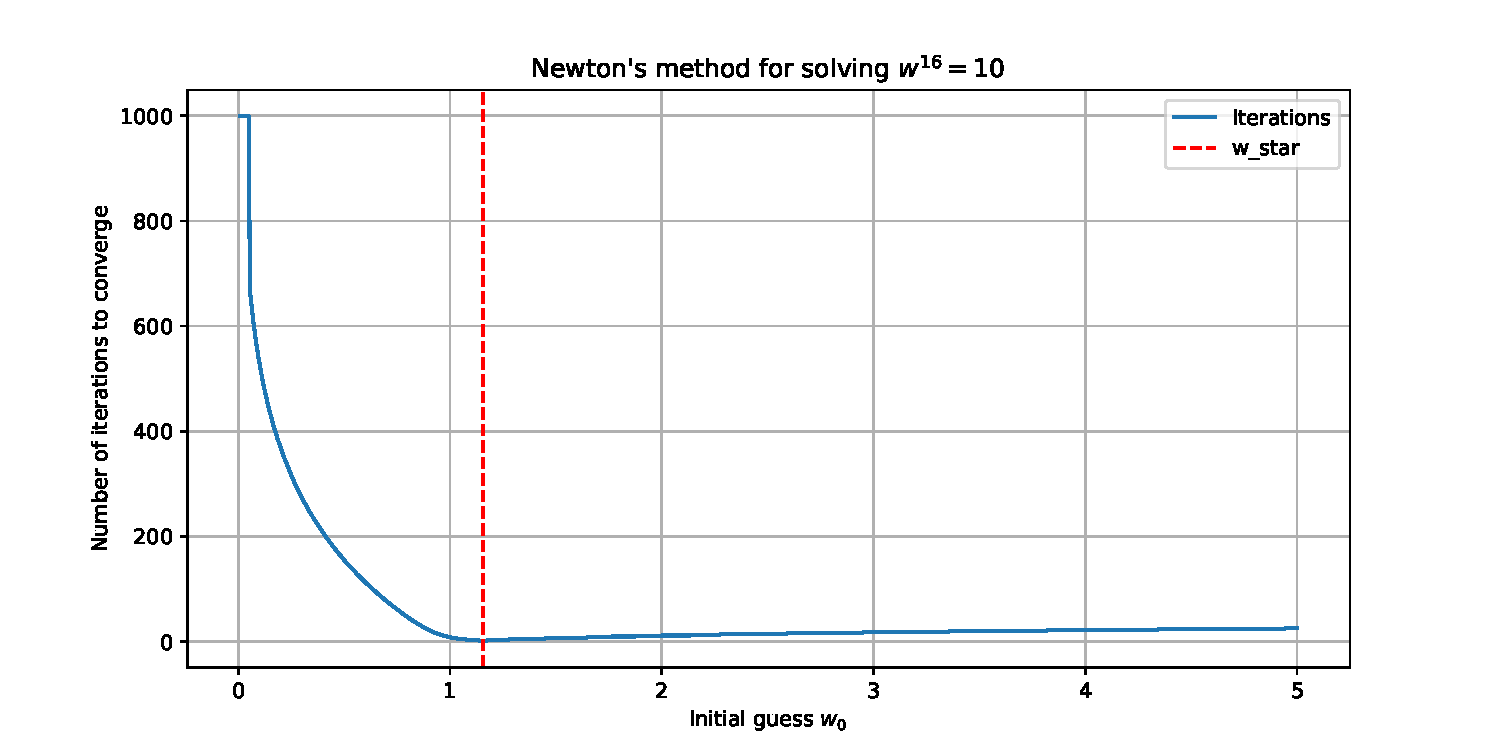
\includegraphics[width=\linewidth]{non-lifted.pdf}
    \caption{Iteration count over initial guess for regular Newton's method}
    \label{fig:linreg}
  \end{subfigure}

  \begin{subfigure}{\textwidth}
    \centering
    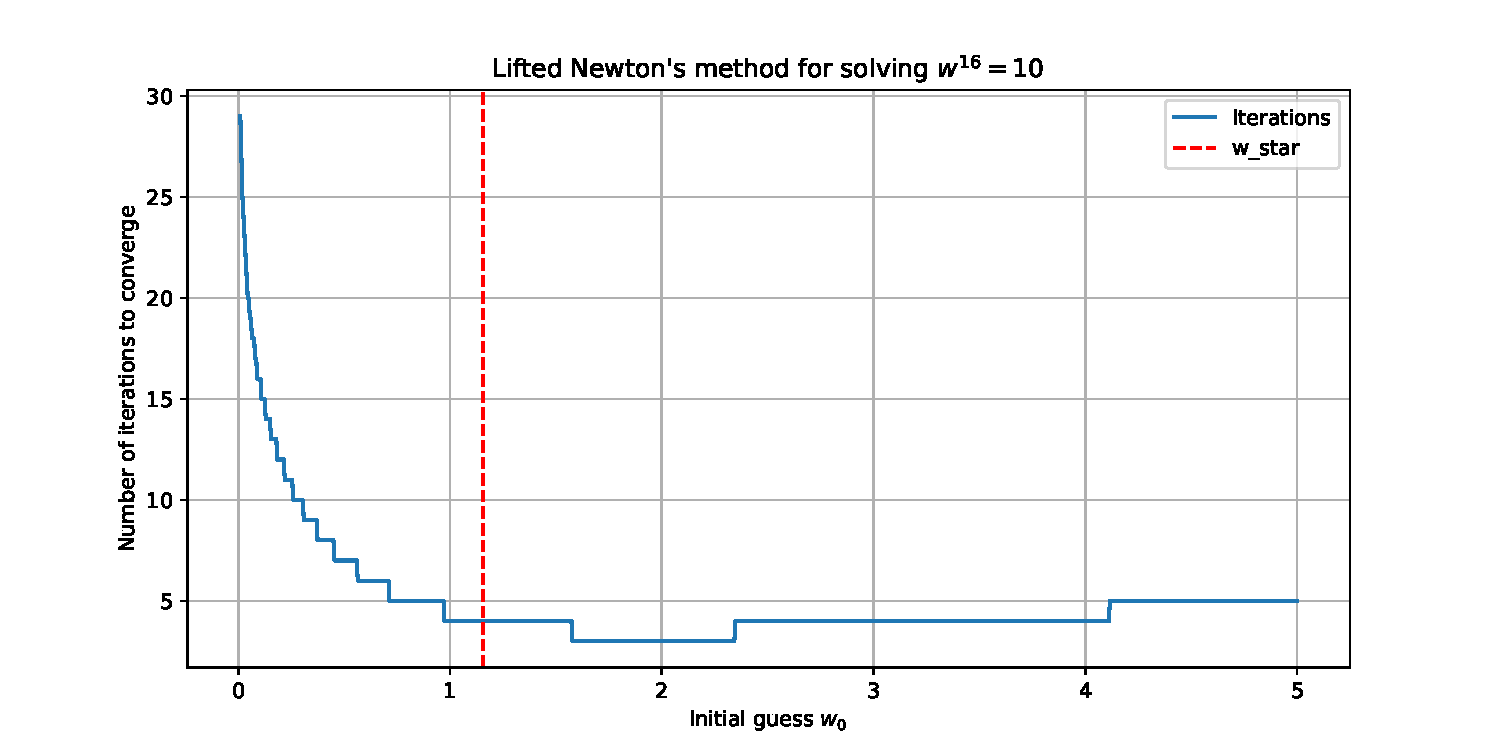
\includegraphics[width=\linewidth]{lifted.pdf}
    \caption{Iteration count over initial guess for lifted Newton's method}
    \label{fig:linregout}
  \end{subfigure}
  \caption{The comparison of the lifted-and non-lifted approach reveals that while the distribution of iterations over initial guesses appears similar in both approaches, the iteration count for the lifted method is consistently more efficient by orders of magnitude. The regular method appears to have its lowest iteration count where the initial guess and solution coincide, while the lifted method interestingly converges faster for an initial guess around $w_0=2$, or slightly above the solution $w^*=\sqrt[16]{10}$. While both methods struggle for low initial guesses, where progress can only be made at an excruciatingly slow pace due to the exponent of $15$ in the function gradient, the lifted method appears to be much more robust to such averse choices of initial value.}
\end{figure}




\end{document}